\documentclass[12pt]{article}
\usepackage{graphicx}
\graphicspath{./figures/}
\usepackage[margin=1.0in]{geometry}
\usepackage{xcolor}
\definecolor{bg}{HTML}{16171e}
%\usepackage[font={color=white,bf}]{caption}
\usepackage{float}
\usepackage{amsmath}
\usepackage{url}
\usepackage{subcaption}
\usepackage{listings}

\title{MCEN 7221/ASEN 5027 Turbulence Project 2}
\author{Duncan McGough}
\date{\today}

\begin{document}
\maketitle

\tableofcontents
\listoffigures
\newpage

\section{Problem 1}
In this project report, Direct Numerical Simulation (DNS) data was taken and analyzed. Two different kinds of simulations were analyzed, one being Homogeneous Isotropic Turbulence (HIT) and the other being Homogeneous Shear Turbulence (HST). 

\subsection{Max and Min Values}
The DNS data for HIT and HST cases was put into a min/max function to find the minimum and maximum values for each velocity component in the HIT and HST fields. In meters per second, the results are:
\begin{lstlisting}
Max HIT u: 0.8576899766921997
Max HIT v: 0.5416799783706665
Max HIT w: 0.7064499855041504
Max HST u: 5.862400054931641
Max HST v: 3.033799886703491
Max HST w: 3.131500005722046

Min HIT u: -0.7590799927711487
Min HIT v: -0.6005899906158447
Min HIT w: -0.7692000269889832
Min HST u: -5.138700008392334
Min HST v: -3.3306000232696533
Min HST w: -2.963900089263916
\end{lstlisting}

One can notice that the extreme values are in the HST case are of greater magnitude than those of the HIT case. In the HIT case, the values are generally smaller and closer together in magnitude, whereas in the HST case it is evident that the u-component has a standout larger velocity whereas the v- and w-components are similar in magnitude. This makes sense due to the nature of the simulation, as the shear has a certain imposed velocity (at least initially) that drives the flow. 

\subsection{3D Isosurfaces}
Three-dimensional isosurfaces can be created and plotted for the HIT and HST cases. When visualized, they appear as in Figure \ref{fig:iso}.

\begin{figure}[H]
\centering
\begin{subfigure}{0.5\linewidth}
\centering
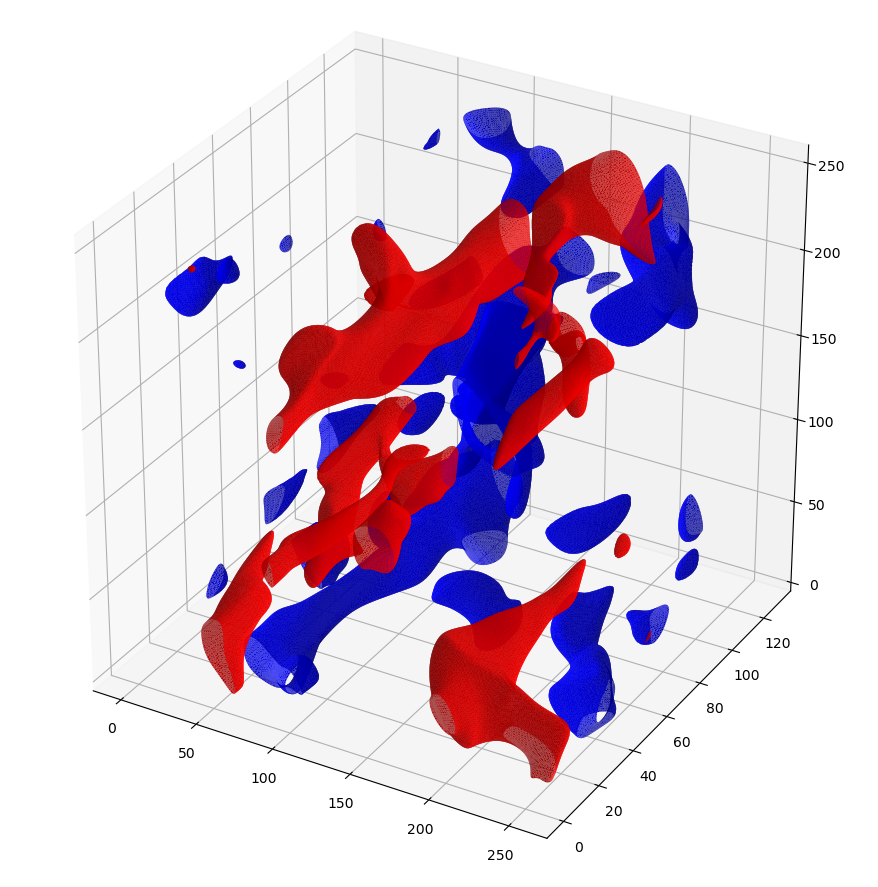
\includegraphics[width=\linewidth]{./figures/12-hit.png}
\caption{HIT}
\end{subfigure}%
\begin{subfigure}{0.5\linewidth}
\centering
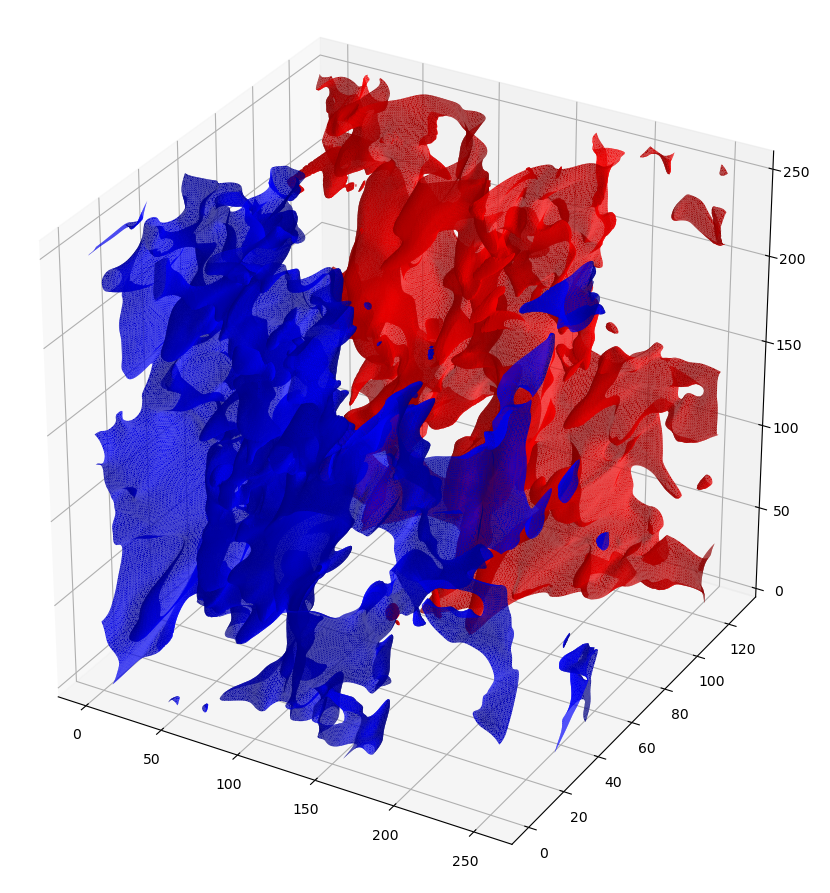
\includegraphics[width=\linewidth]{./figures/12-hst.png}
\caption{HST}
\end{subfigure}
\caption{3D Isosurfaces}
\label{fig:iso}
\end{figure}

The two colors in Figure \ref{fig:iso} represent the maximum and minimum velocities divided by two, respective to the colors blue and red. It is immediately noticeable that the HST case has a distinct division between the maximum and minimum isosurfaces, whereas the HIT case is more uniform. Another distinct feature between the cases is that HIT case has more frequent separate blob entities in a homogeneous formation of isosurfaces whereas the HST case are distinct in their shear layers. 
\subsection{Image Plane Slices}
The data can be sliced at certain planes, leaving 2D slices that can be plotted. In Figures \ref{fig:13-hit} and \ref{fig:13-hst}, the u, v, and w velocity component fields are sliced at k=[1, 128, 256] z-locations. Note that colorbar here is scaled to HST for easy comparison. Increasing slice locations are located in the columns of images whereas different velocity components are the rows of images. It is noted that u-component is the most active and polar with the velocity field in the HST data, as expected. The HIT data is more uniform and homogeneous. An interesting feature of the data is that the k=1 and k=256 planes appear identical. This is due to a repeating boundary condition that is applied to the domain of the simulation. 

\begin{figure}[H]
	\centering
	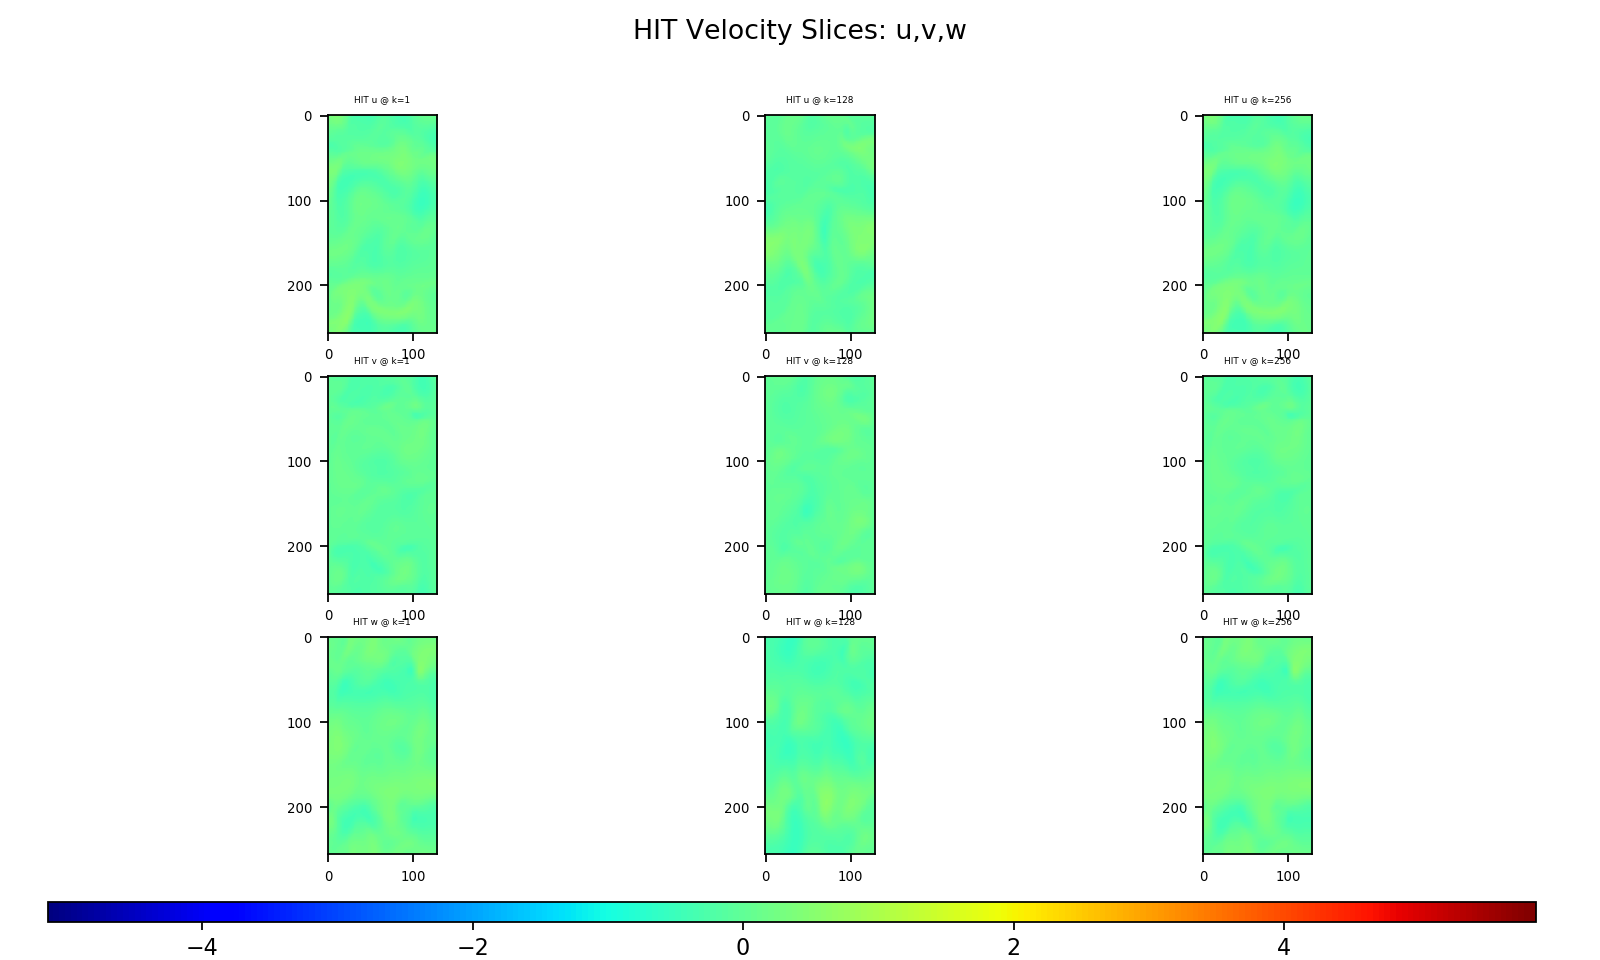
\includegraphics[ width=\linewidth]{./figures/13-hit.png}
	\caption{HIT Velocity Component Slices}
	\label{fig:13-hit}
\end{figure}	

\begin{figure}[H]
	\centering
	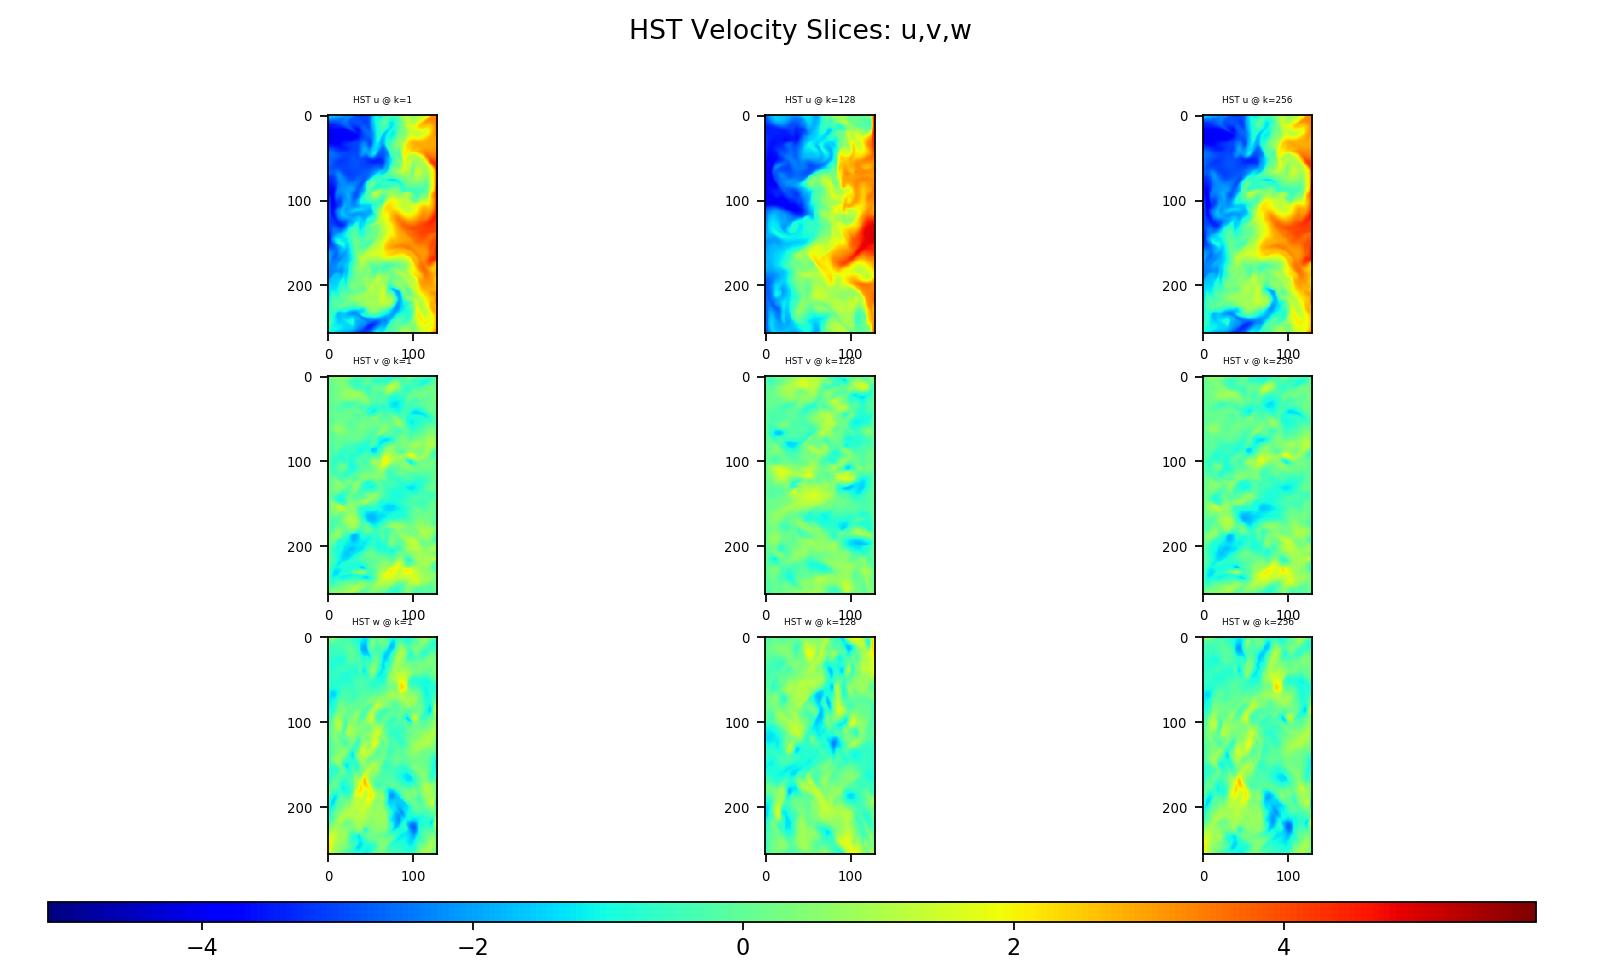
\includegraphics[ width=\linewidth]{./figures/13-hst.png}
	\caption{HST Velocity Component Slices}
	\label{fig:13-hst}
\end{figure}	

\subsection{Spatial Directions}

\subsection{x-z Averages}






%\bibliography{refs}
%\bibliographystyle{ieeetr}

\end{document}
